\documentclass{article}
\geometry{a4paper} 
\usepackage[utf8]{inputenc}
\usepackage{textcomp}
\usepackage{graphicx} 
\graphicspath{{images/}}
\usepackage{amsmath,amssymb,amsthm}  
\usepackage{bm}  
\usepackage[pdftex,bookmarks,colorlinks,breaklinks]{hyperref}  
\hypersetup{linkcolor=black,citecolor=black,filecolor=black,urlcolor=black} % black links, for printed output
\usepackage{memhfixc} 
\usepackage{pdfsync}  
\usepackage{fancyhdr}
\usepackage{enumitem}
\usepackage{cite}
\usepackage{txfonts}
\usepackage{setspace}
\usepackage{siunitx}
\usepackage{lipsum}
\usepackage{natbib}
\usepackage{eucal}
\usepackage{physics}
\usepackage{pst-node}
\usepackage{tikz-cd}
\usepackage{upgreek}
\usepackage{systeme}
\usepackage[toc,page]{appendix}


\pagestyle{fancy}
\newcommand{\tn}[1]{\textnormal{#1}}
\graphicspath{{./images}}
\doublespacing
\newtheorem{definition}{Definition}

\title{Project Report \\
        \large Twistor Theory\\}
\author{FONG Ching}


%\date{}
\begin{document}
\maketitle
\tableofcontents

\section{Abstract}

This paper gives an overview of the twistor theory, which is formulated by
Roger Penrose\cite{originalpaper}. Twistor theory (TT) is one of the many
theories attempting to unite our current best candidate in explaining
gravity - General Relativity (GR) and our best candidate in
explaining small-scale structures - Quantum Field Theory (QFT), as there are
parts of the theories which are incompatible with one another. This paper
is structured as follows, in section I, several abstract mathematical
concepts are introduced to provide the reader with minimum understanding to study
twistor theory. 

\newpage

\vspace*{90px}
\begin{figure}[h!]
\begin{center}
  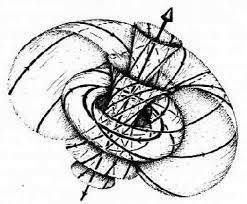
\includegraphics[scale=1.6]{Figures/twistor.jpeg}
\end{center}
\caption{abstract representation of twistor by Roger Penrose.}
\label{fig: twistor pasta}
\end{figure}

\newpage


\section{Introduction}






\subsection{twistor theory in its essence}%
  \label{sub: twistor theory in its essence}
  
Before exploring the mathematical construct behind twistor theory, it 
is best to provide the reader here the overall idea of twistor theory to not
get completely lost in mathematical abstraction. 

Twistor theory aims to look at the traditional spacetime at a different
perspective. In GR, we look at each event in spacetime as a point, in
which one can draw a light cone to define causal relationships and define
the light rays as the null vectors. However, the goal of twistor theory is to
look at this differently, thus Penrose constructed the twistor
space, in which each point in spacetime is now a Riemann Sphere, and the
light rays become points. With this mathematical construct, one will get new
results and provide a different perspective to work on physics of GR and QFT.

\begin{figure}
\begin{center}
  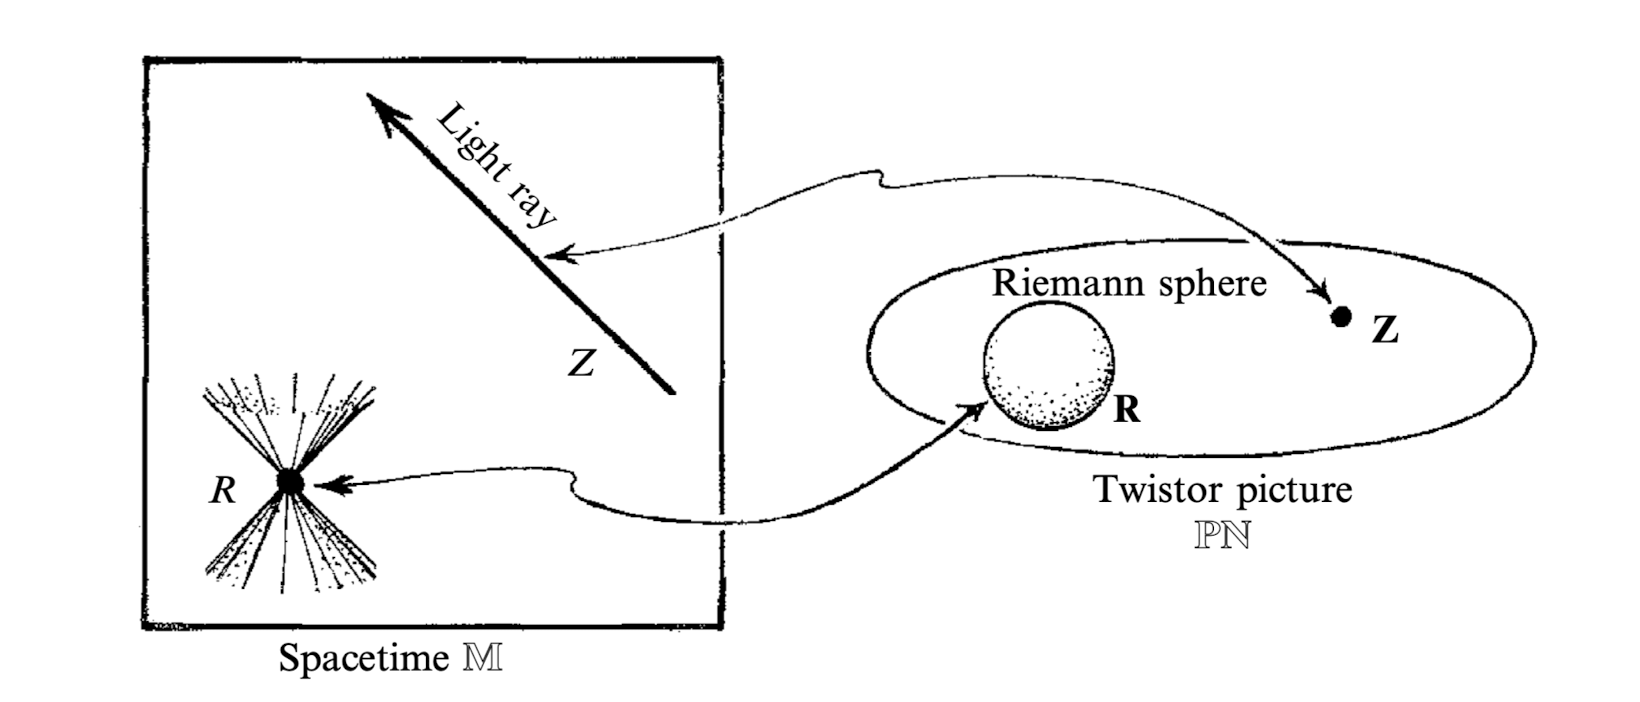
\includegraphics[scale=0.5]{Figures/twistorspacevisual.png}
\end{center}
\caption{shows how one perceives light cone and light ray differently
  in twistor space. Extracted from \cite{road}. }
\label{fig:}
\end{figure}

\section{Mathematical Tools}

In this section, we will briefly review some mathematical constructs
that is required to understand TT.

\subsection{2-spinor representation in Minkowski space}
To describe a point in Minkowski space $ \mathbb{M} $, we can simply use a 
vector $ v^a = (v^0, v^1, v^2, v^3) $, but it is also possible to represent
the space with spinors, in fact, each vector as a geometrical quantity
can be decomposed into two vectors by following:
\begin{align}
  \label{vector to spinor representation}
  v^{\alpha \dot{\alpha}} := \frac{1}{\sqrt{2}} \sigma^{\alpha
  \dot{\alpha}}_{a} v^a = \frac{1}{\sqrt{2} }(\sigma^{\alpha
  \dot{\alpha}}_{0}v^0 + \sigma^{\alpha
  \dot{\alpha}}_{1}v^1 + \sigma^{\alpha
  \dot{\alpha}}_{2}v^2 +  \sigma^{\alpha
  \dot{\alpha}}_{3}v^3   ) =  
  \frac{1}{\sqrt{2} }
  \begin{pmatrix}
  v^0 + v^3 & v^1 - i v^2 \\ 
  v^1 + i v^2 & v^0 - v^3
  \end{pmatrix}
\end{align}
Here $  \sigma^{\alpha
  \dot{\alpha}}_{0}  $ is the 2 dimension identity matrix $ \sigma^{\alpha 
  \dot{\alpha}}_{i}   $, i runs from 1 to 3, refers to the 3 Pauli
  matrices respectively.

This decomposition of a 4-vector into 2 pairs of spinors is called the Weyl
representation\cite{weylrep1998}.

To make the decomposition more mathematically rigorous. We first notice that 
a complex Minkowski space is SO$(4, \mathbb{C}) $ which
locally isomorphic to $ \text{SO}(2, \mathbb{C}) \cross \text{SO}(2, \mathbb{C})
$. This is a stronger statement for the Lie algebra  $
\mathfrak{so}(4, \mathbb{C})$ is isomorphic to $ \mathfrak{sl}(2,
\mathbb{C}) \cross \mathfrak{sl}(2, \mathbb{C})$. Thus we confirm this
the algebraic relationship is valid, we can then identify that the
decomposition is justifiable because vectors belong to SO(4,
$\mathbb{C}$), and spinors belong to  SL$(2,\mathbb{C})$, with 2 spinors
making up one vector SO(4, $ \mathbb{C} $) $\cong $  SL(2, $ \mathbb{C} $)
$ \cross $ SL(2, $ \mathbb{C} $).



\subsubsection{Properties in 2-spinor representation}%
  \label{sub: Properties in 2-spinor representation}
 
 With this 2-spinor formalism, there are few properties that provides
 a better description of previously known physical quantities. 

 First, we observe that the norm of a vector with respect to the metric
 becomes the determinant of the vector in spinor representation.

\begin{align}
  \label{vector element det}
  \eta_{\alpha \beta} v^{\alpha} v^{\beta}  = 2 \text{  det}(v^{\alpha \dot{\alpha}})
\end{align}

Thus in spinor formalism, the null vector is defined when the
determinant of the vector (in 2-spinor representation vanishes),
the only non-trivial cases are thus vectors of the form $
v^{\alpha \dot{\alpha}} = \mu^{\alpha} \mu^{\dot{\alpha}} $ for some
arbitrary non-zero spinors of opposite chirality. This is because these two
spinors of opposite chirality from the
same column vector and leading the determinant to be rank 1, meaning the
column vector spans 1 dimension only, which means it
vanishes.
Note that this property will be used in later sections (namely
the twistor correspondence).   

\subsubsection{Signatures}%
  \label{sub:signature}
  As the name suggests, complexified Minkowski space differs from our
  reality 3+1 by $3 \cross (1 + i) + (1 + i)$, thus in order to recover
  the Minkowski space, we need to do transformations on spinors in $
  \mathbb{M_{C}} $ such that we can recover it back to our usual physical
  spaces, e.g. Lorentzian, and Euclidean space. For this to happen, we need to
  define various operations on the spinors, here we will mention only on
  Lorentzian signature. 


  In order to make sense of the reason behind the imposed constraints, they are
  derived from first finding out how one recovers the signatures, for
  example in Lorentzian signature,
  starting with vectors, we can take Lorentzian space as an example.
  In order for $ x^{\alpha \dot{\alpha}} \in \mathbb{M_{C}}  $ to be in
  Lorentzian signature, i.e. the components $ v^a $ defined in equation
  (1) needs to be all real and with the metric convention diag(-1,1,1,1),
  then we need to require that $ x^{\alpha \dot{\alpha}} $ hermitian,
  i.e. $ x^{\alpha \dot{\alpha}} = (x^{\alpha
  \dot{\alpha}})^{\dagger} $. And with this, it can be derived that the
  constraint for spinors in (1) is equivalent to this.


\subsection{Projective spaces}



To give an overview of the concept of projective spaces. It would be
best first to go through the gist of it with the help of physical
interpretation. 
In its essence, projective spaces describe the space of a n+1 dimensional
space projected onto a n-dimensional space. 

\subsubsection{n = 1 case}%
  \label{sub:n = 1 case}
  

For simplicity, it would be best to start with n = 1. Note that to describe
n = 0 case would not give too much insight since it is trivial to thinking
about, i.e. every point on $ \mathbb{R} $ projects onto the origin. 

The higher dimension space is called the ambient space in most mathematics
literature, and in this case, it is $  \mathbb{R}^{2} \backslash \{0\} $.
The reason for excluding the origin will become apparent later. After
constructing a
line at some arbitrary location (see Figure 2) such that the 
projective space is the space of all straight lines passing through the
origin. Points belonging to the same projective line will condense at
the red horizontal line, that is some form of degeneracy occurs. If we
consider the projective space, it is still a 2D space, however, there is one
less degree of freedom in describing the coordinates in this space.
Explicitly, take any coordinate on $ v = (x, y) \in \mathbb{R}^2 $, we can
equally represent it as $ v = (1, \frac{y}{x}), \textnormal{ with } x \neq 0
$ guaranteed by our previous definition. This seemingly 2D space is exactly
what projective space encodes, and if we focus to the 2-spinor formalism,
spinors are $\mathbb{CP}^{1}$ quantities, and 2-spinors combined can form a
vector of dimension 4. Thus we say, that the 2-spinors double cover a vector.  

\\ 

\begin{figure}[h!]
\begin{center}
  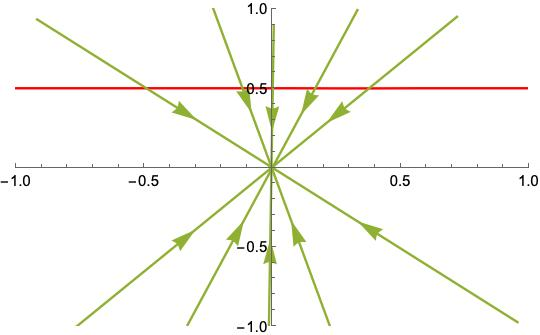
\includegraphics[scale=0.4]{Figures/n=2proj.jpeg}
\end{center}
  \caption{Graphical representation of $\mathbb{R}^2$ onto $\mathbb{R}^2$. One can easily see the all points lying on a given projective line map to the same point that is on the y = 0.5.}
  
  \label{fig:n=2proj}
\end{figure}


\subsection{Spin Group and SO(n)}%
  \label{sub: double cover of Spin Group}
It is non-trivial at first to understand the relationship between the spin group
and SO(n), especially in a more abstract way of representing this concept.
Thus we will start with the representation theory approach

\subsubsection{Abstract description}%
  \label{sub: abstract description of Spin Group and SO(n)}

  In a more abstract setting, there is much less structural
  definition given to Spin(n), and it follows as Spin(n) is a Lie 
  group which is a double cover of the SO(n), coupled with a 
  the short exact sequence between these lie groups as below:
  \\
\begin{figure}[h!]
\begin{center}
    \[ \begin{tikzcd}
      1 \arrow{r} & \mathbb{Z}^2 \arrow{r} & \text{Spin}(n) \arrow{r}
      & \text{SO(n)}
      \arrow{r} & \mathbb{Z}^2 \arrow{r} & 1
\end{tikzcd}
\]
\end{center}
  \caption{shows short exact sequence of the Spin(n) and SO(n) such that
  Spin(n) is well-defined for the discussion. Note that 1 is the trivial
group, and $\mathbb{Z}^2$ is the 2-cyclic group, and both of them are Lie groups
  indeed.}
\label{name: short sequence diagram for Spin Group}
\end{figure}



\subsection{groups and representation theory}%
  \label{sub: groups and representation theory}
  The definition of a group in mathematics 
  since it is a fundamental concept in mathematics. In its essence, a group 
  is a set where its elements within the set obey a set of group 
  axioms and this set encapsulates the idea of symmetry in a 
  more abstract mathematical settings. Certain finite groups, 
  that is groups under certain classifications and constraints, 
  for example U(1) group, exactly corresponds to 
  conserved quantities in physics, related by the Noether 
  theorem (cite here). 

  \subsubsection{SO(3) Group}%
    \label{sub:SO(3) Group}

    SO(3) group is the essence of describing rotation while
    preserving the norm of vector in 3-Space. It is defined as follows:
    \begin{definition}
      A SO(3) group is a set which contains 3x3 matrices as
      elements R that have the constraints: \\ 
      (1) \hspace{0.3cm} $RR^T = 1$, \\ 
      (2) \hspace{0.3cm} $ \textnormal{det}(R) = 1 $
      while the elements in the group obey the usual group axioms,
      that are, (a) closure, (b) associativity, (c) identity, and
      (d) inverse properties. The group multiplication is defined by the
      usual matrix multiplication.
    \end{definition}
   
    To have a brief sense of the reason behind imposing the two
    constraint, (1) is simply the crux of rotation, that the matrix
    and its transpose mapping back to the identity suggests rotation
    along some axis, while (2) is imposed to preserve the norm while
    rotating objects (e.g. vectors, tensors, etc).

  \subsubsection{Representation Theory}%
    \label{sub: Representation Theory}
    
\begin{definition}
  A representation $\pi: G \to GL(V)$ of a group G over a field k is a k-vector space V together
  with an action of G on V by linear maps. Another way to look at it is that it
  is a homomorphism from G to GL(V). 
\end{definition}

Albeit the group theory lets us probe into fundamental physics - conserved
quantities as well as particle pairs in QFT. (cite here) 
It is sometimes too abstract for physicists to work with, in particular, pure abstraction does not help in to prediction of real physical value at all.
 For example, to calculate the matrix element to obtain the cross section for particle decays. 
This is exactly where representation theory comes into play, it deals with
abstract groups with matrices instead,
and this can be done as long as the group we are dealing with is isomorphic
to the matrix group. 

\subsubsection{explicit example of application of representation theory}%
  \label{sub: explicit example of application of representation theory}

\subsection{Fibration}%
  \label{sub:Fibration}
  In this subsection, we will introduce briefly the concept of fibration, which provides a deeper understanding of studying twistor theory. 

We will also provide minimal definitions that are essential to
understanding the definition of fibration. 

  \subsubsection{lift}%
\begin{definition}
  Given a mapping $f: X \to \mathbb{M_C}$,
  and also a map $\pi_1: \mathbb{PS} \to \mathbb{M_C}$, a lift is a map $h:
  X \to \mathbb{PS}$ such that $\pi_1 \circ h = f$. \\ 
  The graphical way to
  represent this is provided below.  
\end{definition}


\begin{figure}[h!]
\begin{center}
    \[ \begin{tikzcd}
       & \mathbb{PS} \arrow{d}{\pi_1} \\%
      X \arrow{r}{f} \arrow[dashed]{ru}{h}& \mathbb{M_{C}} 
\end{tikzcd}
\]
\end{center}
  \caption{shows the commutative diagram such that the definition for
  lifting is established.}
\label{fig: commutative diagram of lift}
\end{figure}

To understand this in a more physical sense. This is to say if a space $
\mathbb{PS} $ can morph into $ \mathbb{M_{C}} $ under some map , and that $ X $ can also
morph into $\mathbb{M_{C}}$ under some map, then the lift is the map where
$X$ morph into $\mathbb{PS}$.  
\subsubsection{homotopy lifting properties (HLP)}%
  \label{sub: homotopy lifting properties (HLP)}
  \begin{definition}
    A mapping $\pi_1: \mathbb{PS} \to \mathbb{M_{C}}$ satisfies the HLP
    for a space X if (1) for every homotopy h:  $ X \cross [0,1] \to
    \mathbb{M_{C}} $
    and (2) for every mapping (or so-called lift) $\tilde h_0: X \to
    \mathbb{M_{C}}$ with $  \tilde h_0 =  \tilde h |_{X \cross \{0\}}
    $, and that $ \tilde h $ is defined such that $ h = \pi_1 \circ \tilde h
    $ (or in words, $\tilde h$ is defined such that $\tilde h$ lifts
    h), and there exists a homotopy $ \tilde h: X \cross [0,1] $.   
      \end{definition}
 \begin{figure}[h!]
\begin{center}
    \[ \begin{tikzcd}
      X \cross \{0\} \arrow{r}{\tilde h_0} & \mathbb{PS} \arrow{d}{\pi_1} \\%
      X \cross [0,1] \arrow{r}{h} \arrow[dashed]{ru}{\tilde h}&
      \mathbb{M_{C}} 
\end{tikzcd}
\]
\end{center}
  \caption{shows the commutative diagram such that the definition for
  HLP is well-established.}
\label{fig: commutative diagram of lift}
\end{figure}

In a more simple manner, the map that takes one space to another exhibits HLP for some
space $X$ when that space $X$ can simultaneously and continuously morph into
the separate two spaces of interest. In this case, $X \cross [0,1]$ can
continuously morph into $\mathbb{PS}$ and $ \mathbb{M_{C}} $. And if one were
to imagine the continuous morphing as a dynamical evolution, $X$ will morph
into the other two smoothly, and form both the spaces. 

\subsection{Sheaf}%
  \label{sub: Sheaf Cohomology}
  In this subsection, we will review the concept and we shall begin with
  presheaves.
  \subsubsection{presheaf}%
    \label{sub:presheaf}
    \begin{definition}
      Let X be a space equipped with a topology, so that (X,
      $\tau$)
      defines a topological space. A presheaf $ \mathcal{F} $ of
      abelian groups on X consist of the data: \\ 
      (a) $\forall$ open sets $ U \subset X $, an abelian group $
      \mathcal{F} $, and \\ 
      (b) $\forall $ inclusion on $ V \subset X $, a morphism of
      abelian groups $ \rho_{U V}: \mathcal{F}(U) \to
      \mathcal{F}(V) $ subject to the conditions: \\ 
      \begin{enumerate}
        \item $ \mathcal{F}(\emptyset) = 0 $   
        \item $ \rho_{UU} = \text{id} $
        \item $ W \subset V \subset U \implies \rho_{UW} =
        \rho_{VW} \circ \rho_{UV} $
      \end{enumerate}
    \end{definition}
The motivation behind this definition is as follows,
suppose the space X is complicated, to begin with, the map
$\mathcal{F}(X)$ maps the complicated topological space X to some abelian
groups, namely the $GL(V^{n})$, such that it will be simpler to do
calculation in this space, this corresponds to (a) in the definition,
with $\mathcal{F}$ specifically being an abelian group. 
Next, it will be logical to map empty set to 0 ( point (b) 1. ) as $
\mathcal{F} $ is meant to capture information on a topological subset, and
empty sets contain no information.
After $\mathcal{F}$ is defined, we can set up $\rho$, which serves as a
tool to cross-check data between individual $\mathcal{F}(U), \forall U
\in X$, and naturally (b) 2. is required. And finally imposing (b) 3. 
, we require the mapping to be sensible in
the sense that it captures the order (or transitive) property of a general
topological space, which is sets are ordered by the operation $ \subset $,
just like numbers are ordered by the operation $ \le $. In the usual context of
presheaf in topology, one would define $\rho$ simply as the restriction
map, i.e. $\rho: \mathcal{F}(U) \to \mathcal{F}(V), \text{with }
\rho(\mathcal{F}(U)) = \rho(\mathcal{F}(U)) \mid_{V}$. 
It would also be beneficial to mention some technical terms here. In
mathematical literature, the space $\mathcal{F}(U), \text{for some } U
\subset X$ is called a stalk (over the set U), and any one element in
the stalk is called a section. 

\subsubsection{Sheaf}%
  \label{sub:Sheaf}
  A sheaf is simply a stronger requirement of presheaf, which is 
its sections are determined by local data.
\begin{definition}
  \leavevmode \\ 
  (1) if U is an open set on X, and $ \{ V_i \} $ are open covers on U, and if $ s \in \mathcal{F}(U)  $ is an element s.t. $ s
  \mid_{v_i} = 0, \forall i $, then s = 0. \\ 
  (2) if U is an open set on X, and $ \{ V_i \} $ are open covers on U. If $s_i \in \mathcal{F}(V_i)$ for each i, s.t. for each i, j,
  $ s_i \mid_{v_i \cap v_j} =  s_j \mid_{v_j \cap v_i} \implies \exists
  ! s \in \mathcal{F}(U) $ s.t. $s \mid_{v_i} = s_i$ for each i. 
\end{definition}

(1) and (2) are encodes similar ideas. For (1), if the sections of open covers
of some subset U are all 0, then globally the section of subset U should be 0
as well. The same thing should happen in the case where the
intersections of the open covers agree in terms of sections, then there
should be one global unique section on subset U such that the individual
covers inside U agrees with this globally defined section.  

\subsection{Complex Objects}%
  \label{sub: Complex Objects}
  In this section, we review various important geometrical objects that is
  important in studying twistor theory or complex manifolds in general.

  \subsubsection{Differential forms on complex manifold}%
    \label{sub: Differential forms on complex manifold}
    Similar to differential forms on real-valued manifolds. One can
    define differential forms on it. However, due to the nature of
    complex geometry, there are differences between them, which require
    a more careful analysis. 
    
    When complex coordinates are allowed, the usual functions that are
    attached to the forms carry complex coordinates as well, which is
    built into the setting of the Kähler manifold,
    see\cite{ballmann2006lectures}. Thus one-forms become $
    \textnormal{d}z = \textnormal{d}x + i \textnormal{d}y $, where $z$
    is some complex coordinate that takes in two real components, and it
    is also possible to form $ \textnormal{d} \bar z =
    \textnormal{d}x - i \textnormal{d}y. $ With this, any
    differential one form can be represented by the linear
    combination of these two, explicitly written as $
    \sum_{j=1}^{n} f_j \textnormal{z}^j + g_j \textnormal{d} \bar z^j $,
    where $f_j \textnormal{ and } g_j$ need to be holomorphic
    functions, which also explains why in literature these forms are
    called holomorphic differential forms. 

    Similar to forms on real numbers. One can define a higher
    dimensional forms, and they are constructed with the same wedge
    the product that is defined in the regular differential geometry, i.e. $
    \Omega^{p,q} = \Omega^{1,0} \wedge \cdots \wedge \Omega^{1,0} \wedge
    \Omega^{0,1} \wedge \cdots \wedge \Omega^{0,1} $, where the one (1,
    0) forms, which in twistor theory are called holomorphic
    forms, are wedged p times, and the (0, 1) forms, which are called
    anti-holomorphic forms in twistor theory, are wedged q times.
    Since the wedge product is nothing but a tensor product combined
    with sign permutation, the total space formed by all forms of total
    degree n is just the direct sum of all combinations of (p, q) form
    that sum up to n, explicitly $ E^n = \bigoplus_{ p+q=n }
    \Omega^{p,q}. $ Finally, one can define a projection map $
    \pi^{p,q}: E^n \to \Omega^{p,q} $ to obtain the (p, q) form from the
    total space, which is simply the trivial projection, that is if the
    total space is spanned by $ E = \textnormal{d}z^3
    \textnormal{d}\bar z^2 \oplus dz $, we can recover the (1, 0) form just by
    ignoring the 1st direct sum space.

    A holomorphic cotangent bundle can also be defined on a complex manifold
    if one were to collect all (1, 0) and (0, 1) forms for each point on
    the manifold, and direct sum them both to obtain such a bundle,
    $ TP^*M = T^{1,0 *}M \oplus T^{0, 1*}M. $

    \subsubsection{Dolbeault operators}%
      \label{sub: Dolbeault operators}
      In this section, we wish to obtain some operators that behave
      like the usual exterior derivative in the real-valued manifold. The
      the result is that one can define two Dolbeault operators, 
      \begin{align}
        \label{dolbeault operators}
        \partial = \pi^{p+1, q} \circ d : \Omega^{p,q} \to
        \Omega^{p+1, q}, \hspace{1cm} \bar \partial_{}^{} =
        \pi^{p, q+1} \circ d : \Omega^{p,q} \to \Omega^{p, q+1} 
      \end{align}. To see them in action, we begin by defining a form 
      \begin{align}
        \label{dolbeault on omega}
        \omega = \sum_{i = 1}^{p} \sum_{j=1}^{q} f_{i, j}
        \textnormal{d}z^i \wedge \textnormal{d} \bar z^j \in
        \Omega{p,q}
      \end{align}
      and act them of both the Dolbeault operators respectively,

      \begin{align}
        \label{dolbeault action}
        \partial_{}^{}\omega = \sum_{i = 1}^{p} \sum_{j=1}^{q}
        \sum_{l=1}^{} \frac{\partial f_{i,j}}{\partial z^l}
        \textnormal{d}z^l \wedge;
        \textnormal{d}z^i \wedge \textnormal{d} \bar z^j\\
        \bar \partial_{}^{}\omega = \sum_{i = 1}^{p} \sum_{j=1}^{q}
        \sum_{l=1}^{} \frac{\partial f_{i,j}}{\partial \bar z^l}
        \textnormal{d}\bar z^l \wedge \textnormal{d}z^i \wedge
        \textnormal{d} \bar z^j,
      \end{align}
      where the summation on l carries up to the number of
      coordinates (arguments) in $f_{i,j}(z^l)$, and from these two
      equations, it can be seen that the Dolbeault operators have the
      properties: 
      \begin{align}
        \label{dolbeault properties}
        \textnormal{d} &= \partial_{}^{} + \bar \partial_{}^{}\\ 
        \partial_{}^{2} = \bar \partial_{}^{2} &= \partial_{}^{} \bar
        \partial_{}^{} + \bar \partial_{}^{} \partial_{}^{} = 0
      \end{align}
      With this, the Dolbeault operators became the promoted
      version of the usual exterior derivative for Kähler
      manifold, in particular, the Dolbeault cohomology, which is
      analogous to de Rahm cohomology, can be
      established\cite{demailly1997complex}. 

      \subsubsection{tangent vectors on complex manifold}%
        \label{sub: tangent basis}
        Other than the complex differential forms on Kähler
      manifold, one can also define the tangent vectors, which
      are called holomorphic tangent vectors, for a given point p on M,
      one can represent the tangent vector at the point p via the
      tangent basis in the holomorphic tangent bundle at p, which is
      nothing but the dual of holomorphic cotangent bundle at p, and it
      becomes $ v = v^i \partial_{i}^{}  + v^j \bar
      \partial_{j}^{} $, where the two partial derivatives are 
\begin{align}
  \label{$partial derivatives on complex manifold}
     \partial_{i}^{} = \frac{\partial  }{\partial
     z^i}\bigg{\mid_p};
     \hspace{1cm} 
       \bar \partial_{j}^{} = \frac{\partial  }{\partial \bar
      z^j}\bigg{\mid_p},
\end{align}
      but not the Dobeault operators that are defined in the
      previous section. The holomorphic tangent bundle form as  
    $ TP^M = T^{1,0 }M \oplus T^{0, 1}M. $

    \subsubsection{Holomorphic delta function}%
      \label{sub:Name}
     Just as we have a delta function in real-valued space, there is a
     corresponding one for complex space, which is defined as,
     \begin{align}
      \label{holo delta function}
       \bar \delta (z) := \frac{1}{2\pi \textnormal{i}}
       \textnormal{d} \bar z \frac{\partial  }{\partial \bar z}
       \bigg{(} \frac{1}{z} \bigg{)} = \frac{1}{2\pi
       \textnormal{i}} \bar \partial_{}^{} \bigg{(} \frac{1}{z}
       \bigg{)}.
     \end{align}, with the property 
     \begin{align}
      \label{delta property}
       \int_D \textnormal{d}z \wedge \bar \delta(z) f(z) = f(0),
     \end{align}
      where D is the boundary enclosing the origin.
\section{Twistor Theory}

With all these mathematical tools equipped, we can begin to unveil
twistor theory, which it is best to start with the definition of twistor
space.


In its essence, twistor theory is the study of fundamental physics,
that is of QFT and GR in the twistor space, which Penrose believed it
to be the right place to study. Thus we will begin with defining the twistor
space.
\subsection{Mathematical structure of Twistor Theory}%
  \label{sub: Mathematical structure of Twistor Theory}
  
\begin{definition}
The structure of twistor theory is that one studies the double fibration of
  the projective spinor bundle $\mathbb{PS} \cong \mathbb{M_{C}} \cross
  \mathbb{CP}^1$ over the complex Minkowski space 
  $\mathbb{M_{C}}$ and twistor 
  space $\mathbb{PT}$, with the map $\pi_1: \mathbb{PS} \to
  \mathbb{M_{C}}$ taking $(x^{\alpha \dot{\alpha}}, \mu^{\beta})
  \in \mathbb{M_{C}} \cross \mathbb{CP}^1 \cong \mathbb{PS} \mapsto
  (x^{\alpha \dot{\alpha}}) \in \mathbb{M_{C}}$, and the map $\pi_2:
  \mathbb{PS} \to \mathbb{PT}$ taking $(x^{\alpha
  \dot{\alpha}}, \mu^{\beta}) \in \mathbb{M_{C}} \cross \mathbb{CP}^1 \cong
  \mathbb{PS} \mapsto (\lambda^{\dot{\alpha}},
  \mu_{\alpha})$ imposing the relations on
  $\lambda^{\dot{\alpha}}, \mu_{\alpha}$ with $
  \lambda^{\dot{\alpha}} = x^{\alpha \dot{\alpha}} \mu_{\alpha} \text{ and }
  \mu_{\alpha} \neq 0,
  \text{ which is so-called the incidence relation}. $      
 \begin{figure}[h!]
\begin{center}
    \[ \begin{tikzcd}
      & \arrow[swap]{ld}{\pi_2} A \arrow{d}{\pi_5} \arrow{rd}{\pi_1} & \\ 
      B & \arrow[swap]{l}{\pi_3} C \arrow{r}{\pi_4} & D
\end{tikzcd}
\]
\end{center}
   \caption{E}
\label{fig: nig}
\end{figure}

\end{definition}
 
 With this definition,
 \begin{align}
  \label{name}
  \mathbb{PS} = \{\mathbb{M_{C}} \cross
   \mathbb{CP}^{1}\}, \mathbb{M_{C}} = \{\mathbb{C}^4\} \text{ and } \mathbb{PT}
   = \bigg{\{}  ( Z  = \mu^{\dot{\alpha}},
 \lambda_{\alpha} ) \in \mathbb{CP}^{3}
\mid 
 \lambda_{\alpha} \neq 0 \hspace{0.1cm}  \bigg{\}}  
 \end{align}, and Z is called a twistor.


 \subsection{Dual Twistor Space}%
  \label{sub: Dual Twistor Space}
  The definition for dual twistor space is very much identical to the
  definition of dual vector spaces. We begin by the previously defined $
  \mathbb{PT}$, and introduce another space so-called dual twistor
  space $ \mathbb{PT}^{\wedge} $ such that it is dual to $\mathbb{PT}$,
  such that elements from $\mathbb{PT}^{\wedge}$ serves as a linear
  mapping $W \in \mathbb{PT}^{\wedge}: Z \in \mathbb{PT} \mapsto
  \mathbb{R}$. And this space is explicitly 
  \begin{align}
    \label{dual twistor space}
    \mathbb{PT}^{\wedge} = \bigg{\{}
    ( W = \tilde\lambda_{\dot{\alpha}}, \tilde\mu^{\alpha}) \in
    \mathbb{CP}^{3} \mid \tilde\mu^{\alpha} \neq 0
    \bigg{\}}, 
  \end{align} 
  where W is the dual twistor
One can define the inner product between dual twistor and twistor as
\begin{align}
  \label{twistor inner product}
  Z \cdot W =  \mu^{\dot{\alpha}} \tilde\lambda_{\dot{\alpha}}  + 
  \lambda_{\alpha} \tilde\mu^{\alpha} = [\mu \tilde \lambda] + \langle \tilde \mu \lambda \rangle.
\end{align}


\subsection{Twistor correspondence}%
  \label{sub: Twistor correspondence}

 At this point, this definition may seem too abstract and in fact takes
quite some time to digest. Indeed, it would be best first to
describe what kind of objects reside in the twistor space, namely points and
Riemann Spheres which exhibit correspondence to null vectors and points in
Minkowski Space. This correspondence is so-called twistor
correspondence.

 Twistor correspondence states that (1) points in complexified Minkowski space, $x^{\alpha
 \dot{\alpha}} \in \mathbb{M_C}$, are Riemann spheres in the twistor
 space; (2) and points in twistor space, $ X =
 (\lambda^{\dot{\alpha}}, \mu_{\alpha}) \in \mathbb{PT} $, are null
 vectors in complexified Minkowski space, $ v^{\alpha
 \dot{\alpha}}_{\text{null}} \in \mathbb{M_{C}} $.

 To see why this is the case, the proof is as follows:


 \begin{proof} 
   For (1), we start by fixing $x^{\alpha \dot{\alpha}} \in
   \mathbb{M_{C}}$, and by the incidence relation, $
   \lambda^{\dot{\alpha}} = x^{\alpha \dot{\alpha}} \mu_{\alpha} $, we
   have $(x^{\alpha \dot{\alpha}} \mu_{\alpha},\mu_{\alpha} ) \in
   \mathbb{PT}$. We then observe that $ \mathbb{PT} \subset 
   \mathbb{C}^4 $, as $ \mathbb{PT} \subset \mathbb{CP}^{3} $, and since
   $ x^{\alpha \dot{\alpha}} $ is fixed, then the only free parameter
   is $ \mu_{\alpha} \subset \mathbb{C}^2 $, and finally, since we start
   with the coordinates in $ \mathbb{PT} $, therefore the
   projective scaling needs to be consider and it becomes $
    (x^{\alpha \dot{\alpha}} \mu_{\alpha},\mu_{\alpha} ) \subset
    \mathbb{CP}^{1}$. Thus a point in $ \mathbb{M_{C}} $ is
    corresponds to a Riemann Sphere ($ \mathbb{CP}^{1} $) in $ \mathbb{PT}
    $. For a more explicit proof, see \cite{adamo2017lectures}.  
   
   

   For (2), we begin by realizing the result of (1), which tells us that
   we can think of a point in $ \mathbb{PT}  $ as the point intersection of
   two Riemann spheres in $ \mathbb{PT} $ (these two spheres just touches
   each other only at one point in $ \mathbb{PT} $). Now, we know that each Riemann sphere
   corresponds to a point in $\mathbb{M_{C}}$ by the result of (1), and
   denote the corresponding points to be $ x, y \in \mathbb{M_{C}}
   $. Since by default these two Riemann spheres in $  \mathbb{PT} $ and two
   points in $ \mathbb{M_{C}} $ are related by the incidence relation.
   We can subtract both equations to get 
   \begin{align}
     \label{x-y incidence}
     (x-y)^{\alpha \dot{\alpha}} \mu_{\alpha} = 0
   \end{align}

   Next, we raise the $ \mu_{\alpha} \text{  with }\epsilon^{\alpha \beta} $, i.e. 
   \begin{align}
     (x-y)^{\alpha \dot{\alpha}} \mu^{\beta} \epsilon_{\beta \alpha} =
     0
   .\end{align}
   since $ \epsilon_{\beta \alpha} $ is an anti-symmetric tensor and thus
   in order to obtain a non-trivial solution for (4), x-y must be
   proportional to $ \mu^{\alpha} $. Thus it becomes,
   \begin{align}
    \label{5}
     (x-y)^{\alpha \dot{\alpha}} = \mu^{\alpha}
     \tilde{\eta}^{\dot{\alpha}} 
   \end{align}  
   where $ \tilde{\eta}^{\dot{\alpha}}$ is any arbitrary dotted spinor. 
    
    But recall that any vector that can be represented by 2 spinors
    of opposite chirality means that it is a null vector in $\mathbb{M_{C}}$, see equation
    (2). Thus (2) is proved 
 \end{proof}

\section{Zero-rest-mass fields}%
  \label{sec:Application}
  In this section, we will look into the correspondence of z.r.m. fields
  in twistor
  theory.

 \subsection{Zero Rest Mass fields on $ \mathbb{M}$}%
  \label{sub: Zero Rest Mass fields on Minkowski}
  The immediate benefit of studying QFT in twistor space is deriving
  the solution of the Zero Rest Mass fields equation with a much simpler
  approach than what the usual QFT does. Though here we will not derive the
  equation from the bottom-up approach, we study for a specific
  example, namely the spin 1 massless field (photon). 

  \subsubsection{geometric objects in spin 1 zero mass field}%
    \label{sub: objects in spin 1 zero mass field}
    First, we know that the spin 1 zero mass field is simply a gauge
    potential $ A_{\mu \nu} $, and with this we can also define
    the field strength (tensor): 
    \begin{align}
      \label{field strength definiton}
       F_{\mu \nu} := \partial_{\mu} A_{\nu} -
    \partial_{\nu} A_{\mu}
    \end{align} 
  If we represent this in the 2-spinor formalism, it becomes
  \begin{align}
    \label{2-spinor field strength}
    F_{\alpha \dot{\alpha} \beta \dot{\beta} } = \partial_{\alpha
    \dot{\alpha}} A_{\beta \dot{\beta}} - \partial_{\beta
    \dot{\beta}} A_{\alpha \dot{\alpha}} 
  \end{align}
 And notice that $ F_{\mu \nu} $ is an anti-symmetric tensor under
 exchange of $ \mu   $ and $ \nu $, which in 2-spinor formalism,
 it will require the field strength tensor to be anti-symmetric upon
 exchange of $ (\alpha \dot{\alpha}) $ and $ (\beta
 \dot{\beta})$. Or equivalently, we need the exchange upon $ \alpha $
 and $ \dot{\alpha}$ indices symmetric, while the exchange upon $ \beta $ and
 $ \dot{\beta} $ asymmetric, or the other way around. And in 2-spinor
 formalism, any asymmetric tensor must be proportional to the 2D levi-civita
 symbol. This is simply because any $ 2 \cross 2 $ anti-symmetric matrix must have
 its diagonal zero, and the skew-diagonals differ by a negative sign (which
 are simply the definition of the asymmetric tensor). Thus, after some
 careful consideration, one would conclude that $ F_{\alpha \dot{\alpha}
 \beta \dot{\beta} }  $ takes the general form:
 \begin{align}
  \label{field strength dual form}
   F_{\alpha \dot{\alpha} \beta \dot{\beta} }  = 
   \epsilon_{\alpha \beta} \tilde \Phi_{\dot{\alpha} \dot{\beta}} +
   \epsilon_{\dot{\alpha} \dot{\beta}} \Phi_{\alpha \beta}, 
 \end{align}
where $ \tilde \Phi_{\dot{\alpha} \dot{\beta}} = \tilde
\Phi_{(\dot{\alpha} \dot{\beta})} :=
\frac{1}{2}F^{\gamma}_{\phantom{\gamma}\dot{\alpha} \gamma \dot{\beta}}; \hspace{1cm}
\Phi_{\alpha \beta} = \Phi_{(\alpha \beta)} := \frac{1}{2}
F_{\alpha \phantom{\dot{\gamma}} \beta
\dot{\gamma}}^{ \phantom{\alpha} \dot{\gamma}}, $

Indeed, the $ \Phi \text{ and } \tilde \Phi $, which are called self-dual
(SD) and anti self-dual (ASD) portions of the field strength respectively, are symmetric tensors under their
own indices and $ \epsilon $
are asymmetric, therefore the resulting field strength is just as what we
required. 

Next, we can obtain the Hodge dual of the field strength tensor, and to do
this in the usual way, we take the transformation 
\begin{align}
  \label{dual field strength in 2 spinor formalism}
       \small{\star} F =
    \frac{1}{2} \epsilon^{abcd} F_{ab} = \epsilon^{\gamma \delta} \tilde
    \Phi^{\dot{\gamma} \dot{\delta}} - \epsilon^{\dot{\gamma}
    \dot{\delta}} \Phi^{\gamma \delta}, 
\end{align} 
where the first equality is the Hodge dual in the regular vector formalism,
and $ \epsilon^{abcd} $ is the 4D levi-civita tensor. From equation
(9), we can see that $\tilde \Phi$ is indeed SD to the Hodge dual of F and $
\Phi $ is ASD to the Hodge dual of F since they give the eigenvalue
of 1 and -1 respectively under the Hodge dual transformation. Also, note
that $ \epsilon^{abcd} = \epsilon^{\alpha \gamma}
\epsilon^{\beta \delta}
\epsilon^{\dot{\alpha} \dot{\delta}}
\epsilon^{\dot{\beta} \dot{\gamma}}
- \epsilon^{\alpha \delta} \epsilon^{\beta \gamma}
\epsilon^{\dot{\alpha} \dot{\gamma}}
\epsilon^{\dot{\beta} \dot{\delta}}$ in 2-spinor formalism.  

At first glance, it would seem there is little correspondence between SD and ASD
to our usual physical quantities, but turns out, that one can make use of the
Maxwell's equation and the Bianchi identity, which in the standard
differential forms are:

\begin{align}
  \label{standard maxwell in differential form}
  \systeme{
               \textnormal{d}F = 0,
   \small{\star} \textnormal{d} \small{\star}F = J\text{,}
  }
\end{align}
to obtain the 2-spinor formalism version of the two identities, which
exhibit the symmetrical form:

\begin{align}
  \label{2-spinor representation of maxwell equation}
  \systeme{
  \partial_{\beta}^{\dot{\alpha}} \tilde
  F_{\dot{\alpha} \dot{\beta}} + \partial_{\dot{\beta}}^{\alpha}
  F_{\alpha \beta} = 0,
  \partial_{\beta}^{\dot{\alpha}} \tilde
  F_{\dot{\alpha} \dot{\beta}} - \partial_{\dot{\beta}}^{\alpha}
  F_{\alpha \beta} = 0
  }
\end{align}
One would realise that SD part corresponds to the positive helicity
polarization of the gauge potential and ASD part corresponds to the negative
counterpart. For a brief review of the helicity states, one can refer to
Appendix A. Now, if we set either one of the SD or ASD part to be 0, one can
recover the Maxwell fields equation and the Bianchi identities respectively,
however, in twistor language, this corresponds to the spin-1
\textit{zero-rest-mass} (z.r.m.) equations: 
\begin{align}
  \label{z.r.m. equations}
  \partial_{\beta}^{\dot{\alpha}} \tilde F_{\dot{\alpha} \dot{\beta}}
  = 0, \hspace{1cm} \partial_{\dot{\beta}}^{\alpha}
  F_{\alpha \beta} = 0.
\end{align}

This decomposition method can be further applied to z.r.m. fields with
any integer or half-integer spin. For the spin-2 case, in other words, the Weyl
Tensor in GR, is well-studied by
Atiyah\cite{atiyah1978self}. In general, a helicity h z.r.m. equations
are
simply: 
\begin{align}
  \label{z.r.m. equation of helicity h}
  h > 0 \hspace{0.5cm} \tilde \phi_{\dot{\alpha_1}
  \cdots \dot{\alpha_{2|h|}}}, \hspace{1cm} \partial_{}^{\beta
  \dot{\alpha_1}} \phi_{\dot{\alpha_1}
  \cdots \dot{\alpha_{2|h|}}} = 0, \\ 
  h = 0 \hspace{0.5cm} \Phi, \hspace{1cm} \square \Phi =
  \partial_{}^{\alpha \dot{\alpha}} \partial_{\alpha \dot{\alpha}}^{}
  \Phi = 0, \\ 
  h < 0 \hspace{0.5cm} \phi_{\alpha_1
  \cdots \alpha_{2|h|}}, \hspace{1cm} \partial_{}^{\alpha \beta
  } \phi_{\alpha_1
  \cdots \alpha_{2|h|}} = 0, 
\end{align}

\subsubsection{conformity of z.r.m. equations}%
  \label{sub:conformity of z.r.m. equations}
 In most physics applications, it is best to have invariant equations,
 that is equations that are invariant under coordinate or conformal
 transformation. For example, Einstein's field equation or the covariant
 form of Maxwell's field equations. It turns out that the z.r.m. equations
 are also conformally invariant. To see why this is true, we can take the
 spin 1 case as an example. 

 We begin by noticing that the minkowski metric under conformal
 transformation becomes $ \eta_{ab} \to \Omega^2(x) \eta_{ab}. $ But since
 $\eta_{ab}$ in 2-spinor representation is nothing but  $\eta_{ab}
 \leftrightarrow \epsilon_{\alpha \beta} \epsilon_{\dot{\alpha}
 \dot{\beta}}$, then each $\epsilon$ should get a factor of: 
 \begin{align}
   \label{levi-civita conformity}
   \epsilon_{\alpha \beta} \to \Omega(x) \epsilon_{\alpha \beta},
   \hspace{1cm} \epsilon_{\dot{\alpha} \dot{\beta}} \to \Omega(x)
   \epsilon_{\dot{\alpha} \dot{\beta}}. 
 \end{align}
 And we know that the field strength tensor $F_{ab} = F_{\alpha \dot{\alpha}
 \beta \dot{\beta}}$ is conformally invariant, and by equation (19), we
 conclude that both the ASD and SD in (23) transforms with a factor of
 $\Omega^{-1}$, and finally given $ \partial_{\alpha \dot{\alpha}}^{}
 \epsilon_{\beta \gamma} = 0$, which results from simply the classic
 anti-symmetrization rule trick, we can figure out that
 $\partial^{\alpha \dot{\alpha}} \to
 \Omega(x)\partial_{}^{\alpha \dot{\alpha}}$, and thus combining both implies
 (23) is indeed conformal invariant.

 A similar argument can be applied to higher helicity z.r.m. equations,
 and in fact, all z.r.m. fields carries a conform factor of
 $\Omega^{-1}$.




\subsection{positive(negative)-frequency quantities}%
  \label{sub:positive(negative)-frequency quantities)}
 Having introduced the idea of SD and ASD quantities, we further package the
 SD and ASD quantities into the more useful objects called positive
 and negative frequency quantities. 

 Sticking with the example on the field
 strength in electromagnetism. After we defined SD and ASD portions of
 the field strength, we can define the two quantities: \\ 
 \begin{align}
  \label{positive/negative frequency objects and zero helicity objects}
   F^+ = \frac{1}{2}(F_{\mu \nu} - i F^{*}_{\mu \nu});
   \hspace{1cm} F^- = \frac{1}{2}(F_{\mu \nu} + i F^{*}_{\mu \nu}) 
 \end{align}
 They are called positive (self-dual) and negative (anti self-dual) frequency parts of the field
 strength tensor respectively.
  In a more general setting, i.e. higher
  rank tensorial equations, such as the Einstein's Field Equation (EFE), one
  can obtain for such two quantities under similar decomposition. 

  Once the helicity objects are defined. We have successfully divide
  $\mathbb{PT}$ into three parts, which is one of the key results in twistor
  theory. Namely, we have $\mathbb{PT}$ divided to the tree subspaces,
  $\mathbb{PN} = \{\textnormal{ set of all zero helicity objects }\}$ =
 Null twistor space,
  $\mathbb{PT^+} = \{ \textnormal{ set of all positive frequency objects }
  \}$ = positive helicity twistor space and 
  $\mathbb{PT^+} = \{ \textnormal{ set of all positive frequency objects }
  \}$ = negative helicity twistor space. 
\begin{figure}[h!]
\begin{center}
  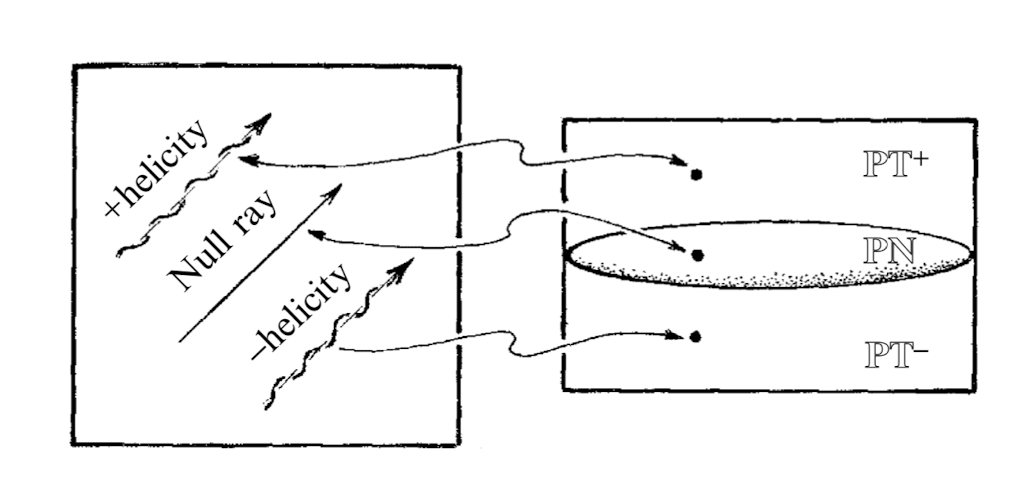
\includegraphics[scale=0.5]{Figures/twistorspace.png}
\end{center}
\caption{shows the decomposition of twistor space into the three subspaces.
  Extracted from \cite{road}.}
\label{fig: twistor space decomposition}
\end{figure}
The above statement can be written out as: 
\begin{align}
  \label{twistor space decomposition}
  \mathbb{PT}^+ = \{ Z \in \mathbb{PT} \mid Z \cdot \bar Z > 0 \},\\ 
  \mathbb{PN} = \{ Z \in \mathbb{PT} \mid Z \cdot \bar Z = 0 \},\\ 
  \mathbb{PT}^- = \{ Z \in \mathbb{PT} \mid Z \cdot \bar Z < 0 \},\\ 
\end{align},
where Z is the twistor mentioned in the previous section.

 \section{The Penrose Transform}%
  \label{sec: The Penrose Transform}
  One major achievement in twistor theory is the Penrose Transform,
  which highly resembles the Radon
  Transform in real integral geometry\cite{radon1986determination},
  the result can simply be stated as any $\pm s$ helicity z.r.m.
  fields on twistor space are equal (corresponds) to  Dolbeault cohomology
  group, or in the mathematical description 

  \begin{align}
    \label{ cohomology group of penrose}
    \{ \phi_{\pm2s-2} \} \cong  H^{0,1} ( \mathbb{PT}, \bigg{\mathcal{O}}(\pm2s-2) ),
    \textnormal{ which obey }\bar \partial_{}^{}f = 0 \textnormal{
    and } 
  \partial_{}^{}f \neq g. 
  \end{align} 
Here, the notation $\bigg{\mathcal{O}}(k)$ is defined as the sheaf of locally holomorphic functions homogenous of weight k on $\mathbb{PT}$, that is $ f(rZ) = r^k f(Z). $ 
In other words, the elements (0, 1)-th cohomology group of weight $
\pm2s\pm2 $
are the positive and negative helicity fields in twistor space. And in other
literatures, one may prefer using sheaf cohomology for a more general
settings, such as twistor space imposed with some signatures, or modified
version of twistor theory\cite{casali2015new}\cite{geyer2014ambitwistor}. 
In this section, the proof behind this correspondence will be lightly
touched upon. 

\subsection{On finding correspondence of z.r.m field in $\mathbb{PT}$}%
 
 Here, we will only prove the correspondence in one direction, i.e. z.r.m.
 equations imply the cohomology group and for the h $<$ 0 case. The other way around is much more
 mathematically involved and it is proved by
 Eastwood, Michael and
 Penrose\cite{eastwood1985generalized}\cite{eastwood1981cohomology}. 

 We begin by observing that fields in $\mathbb{M_{C}}$ are points in
 $\mathbb{M_{C}}$ associated with the corresponding field value, thus through
 twistor correspondence, we immediately see that fields in $\mathbb{PT}$
 cannot be local but in fact, twistor lines (or $\mathbb{CP}^{1}$).
 It would be also intuitive to have the ansatz that the
 correspondence should involve integrating over the entire twistor
 line, or otherwise a part of the data regarding the point in
 $\mathbb{M_{C}}$ is lost. Thus, given a $\phi_{\alpha_1 \cdots
 \alpha_{2s}}(x)$, we need to match (1) the number of spinors
 indices, which are 2s undotted spinor indices, 
 and (2) the 2s symmetrization upon exchanging the
 spinor indices, and (3) the weight (or homogeneity), which is 0 as we have
 established for a z.r.m field. Recall from.The z.r.m. of spin s correspondence in $\mathbb{PT}$ thus becomes, 
 \begin{align}
  \label{spin s z.r.m. field}
   \phi_{\alpha_1 \cdots \alpha_{2s}}(x) = \int_{X} \langle
   \lambda
   \textnormal{ d}\lambda \rangle \wedge \lambda_{\alpha_1} \cdots
   \lambda_{\alpha_{2s}} f(Z) |_{X \cong \mathbb{CP}^{1}}.
 \end{align} 
 If we ignore the constraints on $f$ for the moment, 
 we see that (2) and (3) are not yet satisfied. In fact, there arises one
 more requirement (4) that the integrand needs to be a (1, 1)-form such
 that it makes sense to integrate over X to get the
 correspondence. If we ignore $f$, the number of spinor indices matches as
 2s so $f$ must not contain undotted spinor indices to satisfy (1); the $\lambda_{\alpha_{i}}$ naturally
 provides the symmetrization required in, so $f$ contains no spinor
 indices (2); the weight is 
 2s+2, which can be obtained by counting the number of $\lambda$
 in the equation, so $f$ needs to be of weight -2s-2 under projective
 scaling to satisfy (3); 
 the integral of R.H.S in (29) is a (1, 0)-form provided by the
 $\textnormal{d} \lambda$, so $f$ needs to be a (0, 1)-form to satisfy
 (4). Furthermore, $f$ has to be (5) a holomorphic function such that the
 integral is mathematically valid. 
 With all these consideration from (1)-(5), $f$ is a weight -2s-2 (0,
 1)-form on $\mathbb{CP}^{1}$, therefore, it has the form: 
 \begin{align}
  \label{z.r.m. cohomology representation}
   f(\lambda, \bar \lambda) = f^{\bar \alpha}(\lambda, \bar \lambda)
   \textnormal{d} \bar \lambda_{\bar \alpha}, \hspace{1cm}
   f(r\lambda, \bar r \bar \lambda) = r^{-2s-2} f( \lambda, \bar \lambda ).
 \end{align}
 However, $f$ in equation (30) is still defined in
 $\mathbb{PT}$, thus one needs to impose restriction on this arbitrary holomorphic
 function $f$, namely the restriction from $\mathbb{PT}$ onto
 $\mathbb{CP}^{1}$. This can simply be achieved by treating the
 incidence relation as the restriction map, which pullback $\mathbb{PT}$
 to $\mathbb{CP}^{1}$. In other words, $f$ becomes $ f(Z, \bar Z)|_X =
 f(x^{\beta \dot{\alpha}} \lambda_{\beta}, \lambda_{\alpha},
 \overline{x^{\beta \dot{\alpha}} \lambda_{\beta}}, \bar
 \lambda_{\bar \alpha}) $.
With this we get explicitly a quantity $f \in \Omega^{0, 1}( \mathbb{PT},
\bigg{\mathcal{O}}(-2s-2))$, i.e. a (0, 1)-form on $\mathbb{PT}$
of projective weight -2s-2, thus (29) is recovered. 

We can then proceed to obtain the z.r.m field equation in (19) by taking
derivative on (34) using the incidence relation,
\begin{align}
  \label{name}
  \partial_{}^{\alpha_1 \alpha} \phi_{\alpha_1 \cdots \alpha_{2s}}
  = \int_{X} \langle
   \lambda
   \textnormal{ d}\lambda \rangle \wedge \lambda_{\alpha_1} \cdots
   \lambda_{\alpha_{2s}} \bigg{(} \lambda^{\alpha_1} \frac{\partial
   f}{\partial \mu_{\dot{\alpha}}}\bigg{|}_X + \bar
   \lambda^{\alpha_1} \frac{\partial f}{\partial \bar
   \mu_{\dot{\alpha}}} \bigg{|}_X   \bigg{)}.
\end{align}
The first term contains the contraction $ \lambda_{\alpha_1}
\lambda^{\alpha_1} = \epsilon^{\alpha \beta} \lambda_{\alpha_1}
\lambda_{\alpha_1} = 0 $ using anti-symmetrization. And recall we have
imposed that $f$ to be holomorphic, which means independent on conjugate
variables, or mathematically as $\bar \partial_{}^{} f = 0$, where $\bar
\partial_{}^{}$ is the Dolbeaut operator defined previously, thus the
partial derivative in the second term vanishes, and thus the z.r.m. equation
is recovered. And $f$ is indeed the cohomology class as required. 

\subsection{z.r.m. field structure in $\mathbb{PT}$}%
  \label{sub:z.r.m. forms in }
 After performing a similar procedure in the previous subsection. We would
 come to conclude that the structure of helicity h z.r.m. equations
 are given by the integral formula: 
 \begin{align}
  \label{integral formula}
   h < 0 \hspace{0.5cm} \phi_{\alpha_1 \alpha_{2|h|}} (x) &= \int_X
   \langle \lambda \textnormal{d} \lambda \rangle \wedge
   \lambda_{\alpha_1} \cdots \lambda_{\alpha_2|h|} f|_{X},\\ 
    h = 0 \hspace{0.5cm} \phi(x) &= \int_X \langle \lambda
    \textnormal{d} \lambda \rangle \wedge f|_X,\\ 
    h > 0 \hspace{0.5cm} \tilde \phi_{\dot{\alpha_1} \cdots
    \dot{\alpha_{2h}}} &= \int_X \langle \lambda
    \textnormal{d} \lambda \rangle \wedge \frac{\partial  }{\partial
    \mu^{\dot{\alpha_{1}}}} \cdots \frac{\partial  }{\partial
    \mu^{\dot{\alpha_{2h}}}} f \bigg{|}_X.  
 \end{align}

 Here, we should take the remark that our discussion so far does take
 signatures into account, and upon adopting a signature, one would get a
slightly different cohomology class and thus different constraints
on $f$, the corresponding cohomology class for different signatures,
especially split signature is discussed in.
\cite{aryapoor2012penrose}.

 
 Although Penrose transform cleverly makes use of the powerful tool of
 cohomology in Algebraic Topology to obtain z.r.m. fields equations,
 it is still lacking in finding the gauge potential that is usually
 attached to the z.r.m field. This is where Sparling further developed it into a transform named after himself
 \cite{sparling1977dynamically}.

\section{Ward's correspondence}%
  \label{sec: Nonlinear Penrose transform (Ward's correspondence)}
  The development of the Penrose transform does not end at the Sparling
  transform, it was later Ward started to ponder towards
  generalization of Penrose transform\cite{ward1977self} to implement
  gauge theory into TT. To do so, it would be most natural to begin with
  reviewing ordinary gauge theory in $ \mathbb{M}$. 

  \subsection{Gauge theory in general setting}%
    \label{sub: Gauge theory review}
    In gauge theory, we start by observing the existence of a gauge
    field, say a $A(x)$, and for a gauge field we can defined a
    \textit{gauge connetion} by promoting the partial derivative $\partial_{}^{}
    \to D = \partial_{}^{} + A$. Further defining
    \begin{align}
      \label{twis}
      F_{ab} = [D_a, D_b],
    \end{align}
    that is the Lie bracket of gauge connection as field strength
    tensor, and take the traces of it, a local gauge-invariant quantity
    is formed. Thus with the connection defined, we have a tool to
    erase redundancy in choosing a gauge, making the theory gauge
    invariant after the appropriate promotion of the lagrangian of the
    theory of interest. 

    \subsection{Gauge theory in TT}%
      \label{sub: Gauge theory in TT}
      
    Suppose we do the same on $\mathbb{PT}$. One can start by
    constructing a gauge connection by promoting the Dolbeault operator
    by 
    \begin{align}
      \label{dolbeault connection}
      \bar \partial_{}^{} \to \bar D = \bar \partial_{}^{} + a,
      \hspace{1cm} a \in \Omega^{0,1}(\mathbb{PT}, \mathfrak{g}).
    \end{align} Here $a$ is a (0, 1)-form that takes values in the
    adjoint of the gauge group G, and $\bar D$ is covariant almost
    complex structure in mathematics. This structure can be thought
    of geometrically as the deformation of complex structures in
    $\mathbb{PT}$, i.e. deformation of $\mathbb{PT}$ manifold itself.
    Similarly, we define a quantity, which is referred to as
    anti-holomorphic curvature of the connection 
    \begin{align}
      \label{name}
      F^{(0, 2)} = [\bar D, \bar D] \in \Omega^{0, 2}(
      \mathbb{PT}, \mathfrak{g} ), 
    \end{align}
    and fix the gauge $F^{(0, 2)} = 0$, which corresponds to $ \bar
    D^2 =  0 $, to arrive at the ward's correspondence. It states
    that a connection $\bar D$ obeying $F^{(0, 2)} = 0$, it will
    corresponds to a SD Yang-Mills field on $\mathbb{R}^4$ with gauge
    group $\textnormal{GL}(N, \mathbb{C})$, which these SD gauge fields
    are referred to as \textit{instantons}\cite{schafer1998instantons}. 
  \section{MHV amplitudes in TT}%
    \label{sec:uMHV amplitudes in TT}
    Another major achievement in TT is providing an alternative
    derivation of Feynman rules for pure Yang-Mills theory, known as
    the MHV rules\cite{schwartz2014quantum}, through gauge theory in twistor space. In this
    section, we will look into the tree-level gluon scattering pure
    Yang-Mills theory. 

    \subsection{Tree-level gluon scattering in pure Yang-Mills theory}%
      \label{sub: Tree-level gluon scattering in pure Yang-Mills theory}
      Scattering amplitudes are fundamental to the study of QFT, as it
      is the major observable in experimental particle physics. Amongst
      different gauge theory in QFT, quantum-chromo-dynamics (QCD)
      is notoriously difficult to calculate for the cross-sections
      in this theory. In fact, our current observational evidence
      relies heavily on the leading order (LO) of the perturbative
      expansion in QCD, with the QCD coupling factor $\alpha_s$.
      In fact, the calculation of gluon scattering amplitudes of higher
      order perturbation expansion in QCD is often handled by
      computers, where physicists have developed numerous method
      to compute the
      amplitudes\cite{dixon2016brief}\cite{elvang2013scattering}.
      
      Despite the active research in QCD scattering calculations,
      there are a few mysteries regarding the calculation, one of them
      being the Parke-Taylor formula for calculating $gg \to gg$
      scattering. For background on this scattering calculation, see
      appendix B.  

      \subsection{Parke-Taylor Formula (PTF)}

        The Parke-Taylor Formula essentially gives a way to
        computed colored order MHV amplitude for any number of
        gluons, that is given a fixed Feynman diagram with only the
        color order unfixed, we have the color ordered amplitude as
      \begin{align}
        \label{Parke tay}
        \mathcal{\tilde M} (1^+ \cdots 2^+ \cdots i^+ \cdots j^+
        \cdots n^+) =  \frac{\langle i j \rangle^{4}}{\Pi_{l =
        1}^{n-1} \langle l (l+1) \rangle \langle n 1 \rangle} =
        \frac{\langle \kappa_i \kappa_j
        \rangle^4}{\Pi_{l=1}^{n-1} \langle \kappa_{l}
        \kappa_{l+1} \rangle \langle \kappa_{n} \kappa_1
        \rangle}, 
      \end{align} 
      where the first and second equality are of the same
      representation (spinor helicity formalism) but the second is to
      emphasize that it is referring to the helicity states of the
      gluon particles. The denominator product is also named the
      cyclic product overall helicity particle states. Initially,
      this formula is obtained by induction on n points gluon
      diagrams, though later Nair\cite{nair1988current}, speculated that this can be derived
      alternatively from twistor theory.

      \subsection{Alternative derivation of Parke Taylor formula}%
        \label{sub: Alternative derivation of Parke Taylor formula}
       
       First, we take any (n-2) positive helicity gluon
       representatives via Penrose transform denoted as $ f^{(1)}
       \in H^{0,1}(\mathbb{PT}, \bigg{\mathcal{O}(0)})$ and $ f^{(-1)}
       \in H^{0,1}(\mathbb{PT}, \bigg{\mathcal{O}}(-4)) $ . And then we take 2
       negative gluon helicity

       Then the Parke-Taylor formula in $\mathbb{PT}$
       representation becomes, 
       \begin{align}
        \label{twis}
         \textnormal{PTF in $\mathbb{PT}$} =
         \int_{\mathbb{M} \cross \mathbb{CP}^{n}} \textnormal{d}^4
         x \bigg{(} \prod_{k = 1}^{n} \frac{D \lambda_k}{\langle
         \lambda_k \lambda_{k+1} \rangle} \bigg{)} \langle
         \lambda_i \lambda_j \rangle^4 f^{(-1)}_i \mid_X
         f^{(-1)}_j \mid_X \prod_{l \neq i, j} f^{(1)}_j \mid_X,
       \end{align} 
      Sometime after this discovery by Nair, 
      Witten\cite{witten2004perturbative} further extended his work to
      what is known as Witten's conjecture.

      \subsection{Witten's conjecture}%
        \label{sub: Witten's conjecture}
        Witten's conjecture states essentially that the entire
        tree-level S-matrix of Yang-Mills theory could be written
        in terms of holomorphic functions from $ \mathbb{CP}^{1}
        \hookrightarrow  \mathbb{PT} $. Simply stated, any tree-level
        The S-matrix of pure Yang-Mills theory (e.g. QCD) can be
        written compactly by a single formula, but not restricted
        to only MHV amplitude. The conjecture was proven to be true
        and the formula is now known as Roiban-Spradlin-Volovich
        (RSV) formula \cite{roiban2004tree}.

        \begin{align}
          \label{name}
          A_n = i(2\pi)^4
          g^{n-2}_{\textnormal{YM}}\sum^{n-3}_{d=1} \int
          \textnormal{d} \mathcal{M}_{n,d} \prod^n_{i=1} \delta^2
          (\lambda_i^{\alpha}- \xi_i P^{\alpha}_i) \prod_{k=0}^{d}
          \delta^2 \bigg{(} \sum_{i=1}^n \xi_i \sigma_i^k \tilde
          \lambda_i^{\dot{\alpha}} \bigg{)} \delta^4 \bigg{(}
          \sum_{i=1}^n \xi_i \sigma_i^k \eta_i A
          \bigg{)}
        \end{align}, where $A_n$ denotes the partial amplitude of
        the color-stripped n-particle in the corresponding Yang-Mills
        theory, $(\lambda_i^{\alpha}, \tilde
        \lambda_i^{\dot{\alpha}}, \eta_{iA})$ denotes the i-th
        particle positive ($\lambda$) and negative ($\tilde
        \lambda$) chirality states, just as defined in the
        standard spinor helicity notation, $\eta_A$ denotes the
        4-component Grassman coordinate of $\mathcal{N} = 4$
        superspace. degree $d$ is given by $ d = \frac{1}{2}( n -
        \sum h_i -2 ) $. The integration measure is given by 
        \begin{align}
          \label{integration measure}
          \textnormal{d} \mathcal{M}_{n,d} = \frac{d^{2d+2}a d^n
          \sigma d^n \xi}{\textnormal{vol}(\textnormal{GL}(2))}
          \prod_{i=1}^{n} \frac{1}{\xi_i (\sigma_i -
          \sigma_{i+1})}. 
        \end{align}

        \section{Conclusion}%
          \label{sec:Conclusion}
          To summarize, TT is one of the candidates in QG, albeit
          having received much less attention from the others,
          namely, string theory and LQG. Nonetheless, it still
          provides profound insight in understanding fundamental
          physics, to both QFT and GR. For example, 
          Ward's correspondence to QFT and Penrose transform to
          both QFT and GR. It even serves to provide a useful
          platform for string theory, in fact, string theorists
          have developed incorporated twistor space to string
          theory, which further
          become the ambitwistor
          theory\cite{geyer2014ambitwistor}. The key point of TT is
          that rather than developing theories in just the
          ordinary Minkowski space, which theorists have been
          doing ever since the discovery of GR, working in Twistor
          space often provides surprising results that we have no
          access to previously. Thus TT is worth remarking as not
          just as a candidate to QG but to theoretical physics
          that involves QFT or GR in general. 

 \begin{appendices}


\section{Massless spin 1 particle}%
  \label{sec: Massless spin 1 particle}

  In this appendix, the minimum background introduction to the theory of
  massless spin 1 particles is provided.
 The lagrangian to describe massless spin 1 particle is as follows:

 \begin{align}
  \label{massless spin 1 lagrangian}
   \mathcal{L} = - \frac{1}{4} F_{\mu \nu} F^{\mu \nu}
 \end{align},
 with $ F_{\mu \nu} = \partial_{\mu} A_{\nu} - \partial_{\nu} A_{\mu}  $.
 Since typically we know that photons are massless spin 1 particles,
 and thus we can associate the theory with electromagnetic wave theory and
 conclude that $ F_{\mu \nu} $ is the field strength tensor, and $ A_{\mu} $
 is the gauge potential.

 One result of this lagrangian is that the potential is invariant
 under U(1) transformation, in other words, it exhibits U(1) symmetry.
 To show this, we can perform the transformation
\begin{align}
  \label{U(1) transformation on gauge potential}
  A_{\mu}(x) \to A_{\mu}(x) + \partial_{\mu} \alpha(x),
\end{align}
for any scalar function $ \alpha(x) $.
With the Euler-Lagrange equation, one can obtain the EOMs
\begin{align}
  \label{EOM of gauge potential} 
  \box A_{\mu} - \partial_{\mu}(\partial_{\nu} A_{\nu}) = 0.
\end{align}

Further solving the equation, one will eventually obtain Fourier
space the solution of $ A_{\mu} $ as

\begin{align}
  \label{solution form of gauge potential}
  A_{\mu}(x) = \int \frac{d^3 p}{(2 \pi)^3} \frac{1}{\sqrt{2 \omega_p}}
  \sum_{i=1}^{2}( \epsilon^{i}_{\mu}(p) a_{p,i} e^{-ipx} +
  \epsilon^{i \star}_{\mu}(p) a^{\dagger}_{p,i} e^{ipx} )
\end{align}
  where $a_{p,i}, a^{\dagger}_{p,i}$ are the annihilation and creation operators
  for momentum p and i-th component, $ \epsilon^i_{\mu}  $ and $
  \epsilon^{\star i}_{\mu} $ are the basis for $ A_{\mu} $. Here we have
   chose 
  the standard gauge (coordinate choice) with $ p^{\mu} = (E, 0, 0 ,E), $
  in the z-direction. It is also worth mentioning that $
   \epsilon^{*}_{\mu} \epsilon^{\mu}  = -1 $ and $ p_{\mu} ϵ^{\mu} =
   0$ 

  For further reading, see \cite{schwartz2014quantum}. 

\section{$gg \to gg$ scattering amplitude in Pure Yang-Mills theory}%
  \label{sec:$gg \to gg$ scattering amplitude in Pure Yang-Mills theory}
We begin by writing down the matrix element of $gg \to gg$ simply using the
   Feynman Diagram and Feynman Rules. In which, we obtain 
   the following, 
  \begin{align}
    \label{gg scatter}
    i\mathcal{M}_s (p_1 p_2 \to p_3 p_4) &= -i
    \frac{g^2_s}{s}f^{abe}f^{cde}[(\epsilon_1 \cdot
    \epsilon_2)(p_1 - p_2)^{\mu} + \epsilon^{\mu}_2(p_2 + q)\cdot
    \epsilon_1 + \epsilon^{\mu}_1 (-q - p_1) \cdot \epsilon_2]\\ 
    &\hspace{1.5cm} \cross [(\epsilon^{*}_4 \cdot \epsilon^{*}_3) (p_4
    - p_3)^{\mu} + \epsilon^{*\mu}_3 (p_3 + q) \cdot
    \epsilon^{*}_4 + \epsilon^{*\mu}_4(-q - p_4) \cdot
    \epsilon^{*}_3],  
  \end{align}
where conservation of momentum tells $ q = p_1 + p_2 = p_3 + p_4 $, and
$\epsilon$ refers to the polarizations, $g$ is the strong interaction
coupling constant, s is the s channel Mandelstam variable. 
However, this is just one of the many diagrams to obtain $gg \to gg$, if we
consider all possible diagrams that contribute to the final averaged
matrix amplitude, we need to calculate 1000 more of these diagrams,
with each diagram having any of the different combinations of
polarizations (abbreviated as pols.), crossed or uncrossed diagrams, and color
factors (abbreviated as cols.). 
The resulting averaged matrix element square though takes the simple form, 

\begin{align}
  \label{simple gg scattering}
  \frac{1}{256} \sum_{\textnormal{pols. cols.}} | \mathcal{M} |^2 = g^4_s
  \frac{9}{2} (3 - \frac{tu}{s^2} - \frac{su}{t^2} -
  \frac{st}{u^2}),
\end{align} where s,t and u correspond to the s, t, and u Mandelstam
variables.


   \begin{figure}[h!]
\begin{center}
  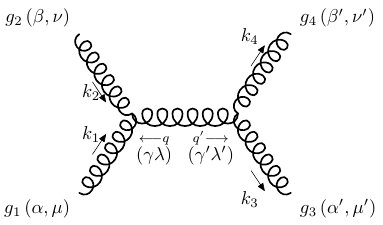
\includegraphics[scale=0.5]{Figures/gg_scatter.jpg}
\end{center}
\caption{shows the Feynman diagram of one $gg \to gg$ scattering channel.
  Extracted from \cite{griffiths2020introduction}.}
\label{fig: gg scatter}
\end{figure}

  

In this section, we will not try to recover the (48) but instead give a rough
picture of how to obtain the equation. The next step is to represent the
momentum quantity $p$ in spinor formalism, which we adopt the usual spinor-helicity formalism,
   that is the convention used in \cite{dixon2016brief} and
  \cite{schwartz2014quantum} chapter 27.1. We then make use of 4-momentum
  conservation and decomposition of spinors, one can obtain the Schouten
  identity. 

  The remarkable result of adopting this formalism is that since
  $\epsilon_{\mu} \epsilon^{\mu} = 0.$, which behaves exactly as $p_{\mu}
  p^{\mu} = 0.$ We can choose a reference momentum such that the 
  polarizations of positive and negative helicity have the
  representation as 
      \begin{align}
    \label{spinor helicity formalism}
        [\epsilon^-_p(r)]^{\alpha \dot{\alpha}} = \sqrt{2}
        \frac{p\rangle [r}{[pr]}, \hspace{1cm}  [\epsilon^+_p(r)]^{\alpha \dot{\alpha}} = \sqrt{2}
        \frac{r\rangle [p}{\langle pr \rangle}.
   \end{align}
  The notation of the spinor helicity formalism and the notation in 2-spinor
  formalism follows as (by taking $v^{\alpha \dot{\alpha}} =
  \lambda^{\alpha} \lambda^{\dot{\alpha}}$)
  \begin{align}
    \label{co}
    \lambda^{\alpha} = v\rangle, \hspace{0.5cm} \lambda_{\alpha}
    = \langle p, \hspace{0.5cm} \tilde \lambda_{\dot{\alpha}} = v],
    \hspace{0.5cm} = [v.
  \end{align}
We will arrived at the result $ \epsilon^+ \cdot \epsilon^+ =\epsilon^- \cdot
\epsilon^- = \epsilon^{\pm} \cdot p = 0   $  
Under this representation, we will conclude that amplitudes that only have 2
positive and 2 negative helicities on the 4 legs remain, whereas the rest all
vanishes. This significantly reduces the calculation, and the corresponding
remnant diagrams are called maximum helicity violating (MHV) amplitudes.

Further calculation under this formalism on the color ordering of the $gg \to
gg$ amplitude will yield the famous Parke-Taylor formula. 


\end{appendices}


\bibliographystyle{unsrt}
\bibliography{references.bib}
        
\end{document}


